\section{Results}

Table~\ref{tab:hard_reentry_results} reports selected-target correctness as percentages of the visible-target interval. Figure~\ref{fig:result_ratios} visualises the same comparison, and Figure~\ref{fig:qualitative_hard_reentry} shows a qualitative hard re-entry example.

\begin{table}[t]
\centering
\caption{Selected-target correctness on the hard re-entry sequence. Values are percentages of the visible-target interval.}
\label{tab:hard_reentry_results}
\begin{tabular}{llccc}
\toprule
Tracker & Variant & Correct & Wrong & Lost \\
\midrule
ByteTrack & Raw & 68.7 & 11.5 & 19.8 \\
ByteTrack & TIM-MARS & \textbf{96.9} & 1.5 & \textbf{1.6} \\
DeepSORT-MARS & Raw & 92.8 & \textbf{0.0} & 7.2 \\
DeepSORT-MARS & TIM-MARS & 92.3 & 5.1 & 2.6 \\
OCSORT & Raw & 48.7 & 35.6 & 15.7 \\
OCSORT & TIM-MARS & 67.2 & 11.9 & 20.9 \\
\bottomrule
\end{tabular}
\end{table}

\begin{figure}[t]
\centering
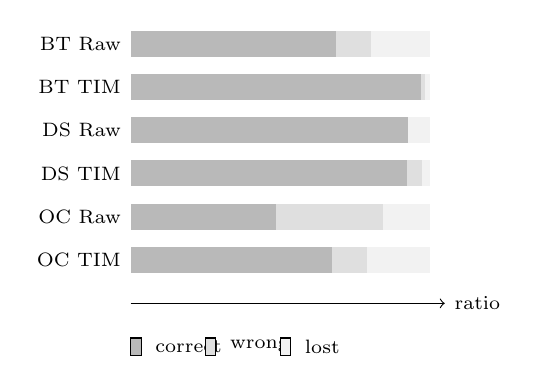
\begin{tikzpicture}[
    x=38mm,
    y=5.5mm,
    font=\scriptsize
]
\draw[->] (0,0) -- (1.05,0) node[right] {ratio};

\node[anchor=east] at (0,6) {BT Raw};
\fill[gray!55] (0,5.7) rectangle (0.687,6.3);
\fill[gray!25] (0.687,5.7) rectangle (0.802,6.3);
\fill[gray!10] (0.802,5.7) rectangle (1.000,6.3);

\node[anchor=east] at (0,5) {BT TIM};
\fill[gray!55] (0,4.7) rectangle (0.969,5.3);
\fill[gray!25] (0.969,4.7) rectangle (0.984,5.3);
\fill[gray!10] (0.984,4.7) rectangle (1.000,5.3);

\node[anchor=east] at (0,4) {DS Raw};
\fill[gray!55] (0,3.7) rectangle (0.928,4.3);
\fill[gray!25] (0.928,3.7) rectangle (0.928,4.3);
\fill[gray!10] (0.928,3.7) rectangle (1.000,4.3);

\node[anchor=east] at (0,3) {DS TIM};
\fill[gray!55] (0,2.7) rectangle (0.923,3.3);
\fill[gray!25] (0.923,2.7) rectangle (0.974,3.3);
\fill[gray!10] (0.974,2.7) rectangle (1.000,3.3);

\node[anchor=east] at (0,2) {OC Raw};
\fill[gray!55] (0,1.7) rectangle (0.487,2.3);
\fill[gray!25] (0.487,1.7) rectangle (0.843,2.3);
\fill[gray!10] (0.843,1.7) rectangle (1.000,2.3);

\node[anchor=east] at (0,1) {OC TIM};
\fill[gray!55] (0,0.7) rectangle (0.672,1.3);
\fill[gray!25] (0.672,0.7) rectangle (0.791,1.3);
\fill[gray!10] (0.791,0.7) rectangle (1.000,1.3);

\node[anchor=west] at (0.05,-1.0) {correct};
\draw[fill=gray!55] (0,-1.2) rectangle (0.035,-0.8);
\node[anchor=west] at (0.30,-1.0) {wrong};
\draw[fill=gray!25] (0.25,-1.2) rectangle (0.285,-0.8);
\node[anchor=west] at (0.55,-1.0) {lost};
\draw[fill=gray!10] (0.50,-1.2) rectangle (0.535,-0.8);
\end{tikzpicture}
\caption{Stacked selected-target correctness ratios. TIM-MARS strongly reduces wrong-target output for ByteTrack and OCSORT.}
\label{fig:result_ratios}
\end{figure}

\begin{figure*}[t]
\centering
\begin{tabular}{cccc}
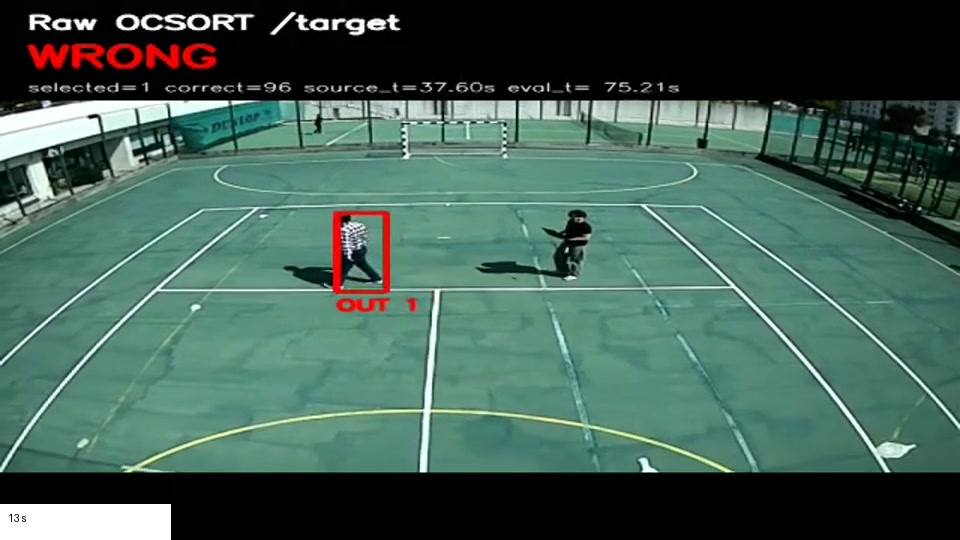
\includegraphics[width=0.235\textwidth]{figures/qual_raw_wrong_crop.jpg} &
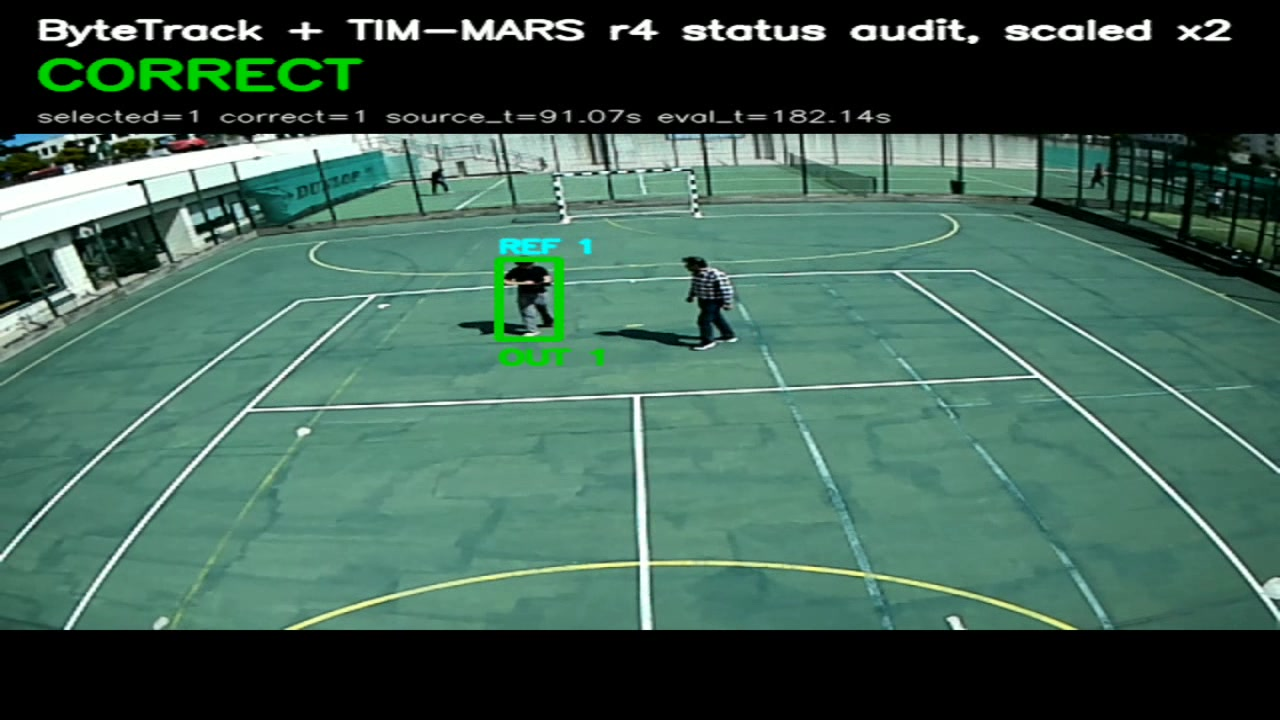
\includegraphics[width=0.235\textwidth]{figures/qual_tim_safe.jpg} &
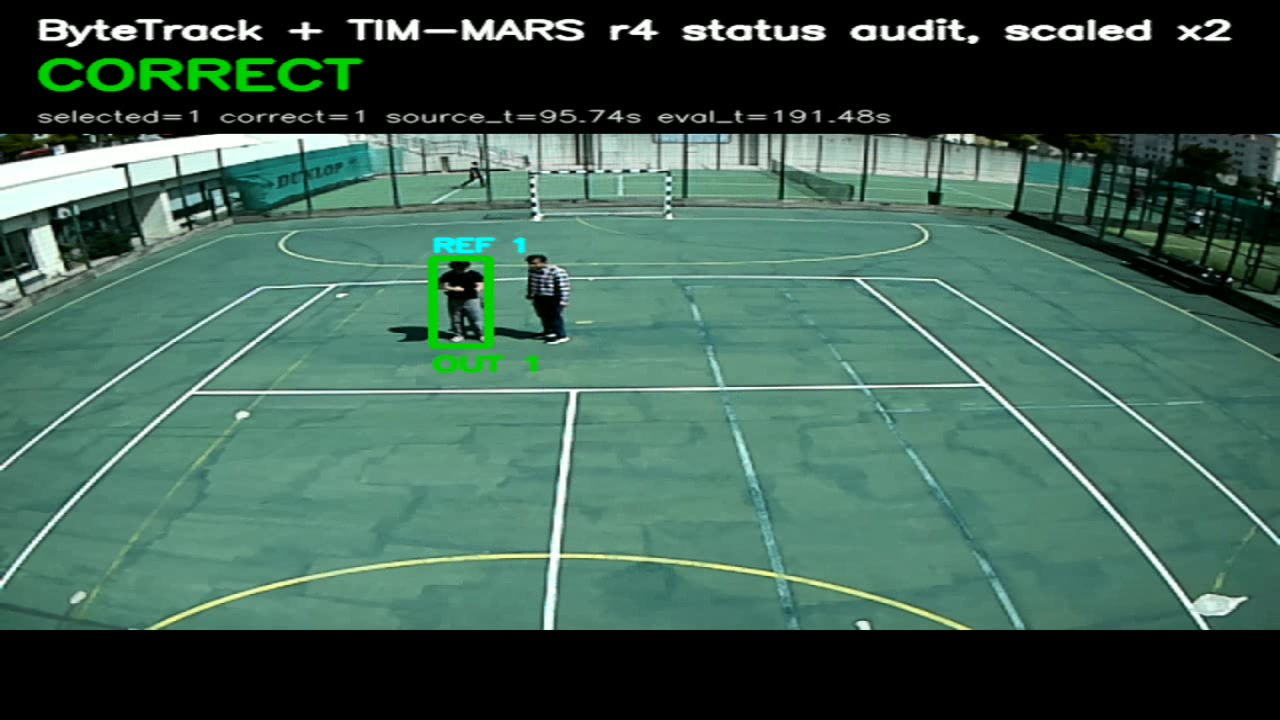
\includegraphics[width=0.235\textwidth]{figures/qual_reentry.jpg} &
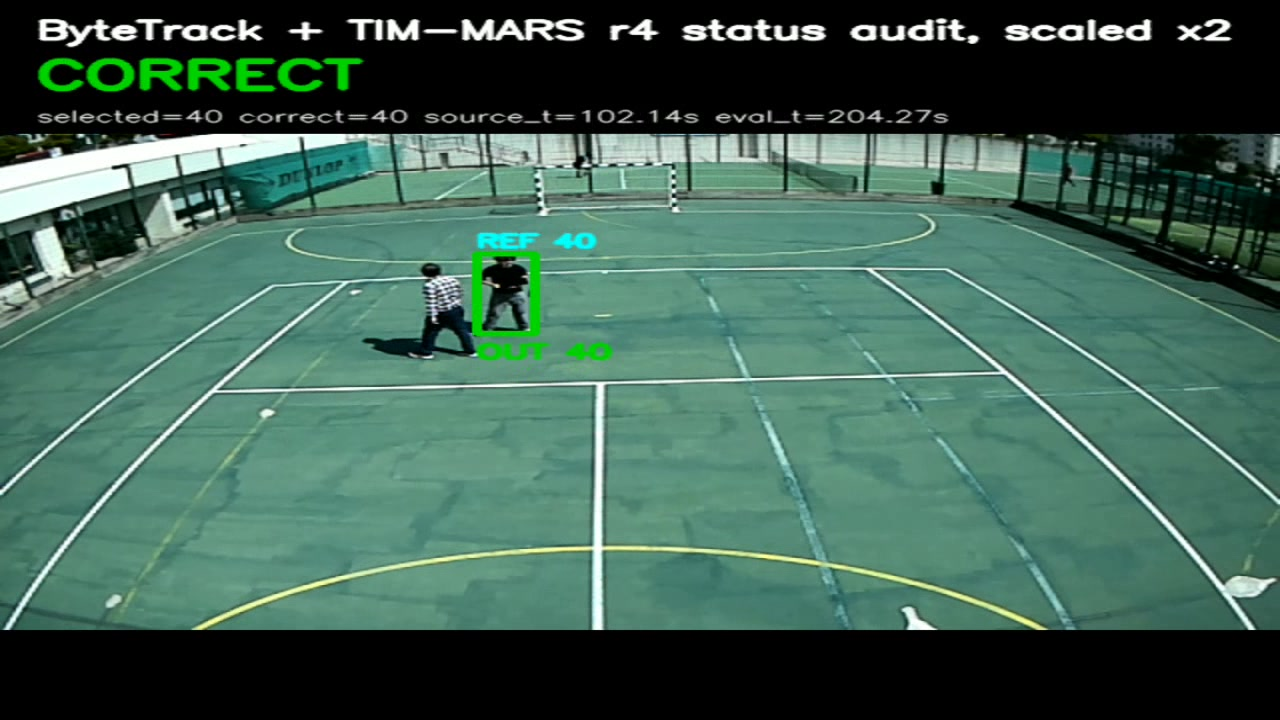
\includegraphics[width=0.235\textwidth]{figures/qual_reacquired.jpg} \\
(a) Raw OCSORT error &
(b) TIM-MARS correct selection &
(c) Close re-entry ambiguity &
(d) Correct identity recovery
\end{tabular}
\caption{Qualitative examples from the hard re-entry sequence. Panel (a) shows a representative raw selected-target failure, where the output persists on the wrong person. Panels (b)--(d) show ByteTrack + TIM-MARS maintaining and recovering the intended target identity after close interaction, even when the numeric tracker ID changes.}
\label{fig:qualitative_hard_reentry}
\end{figure*}


ByteTrack benefits most from TIM-MARS. Correct selected-target output increases from 68.7\% to 96.9\%, while wrong-target output decreases from 11.5\% to 1.5\%. Lost-target output also decreases from 19.8\% to 1.6\%. This indicates that the base tracker had recoverable identity instability and that TIM-MARS improved both safety and continuity.

DeepSORT-MARS is already a strong raw baseline, with 92.8\% correct output and 0.0\% wrong output. Adding TIM-MARS reduces lost output from 7.2\% to 2.6\%, but introduces 5.1\% wrong output. Under the adopted safety rule, this is not a strict improvement.

OCSORT also benefits from TIM-MARS in terms of safety. Wrong-target output decreases from 35.6\% to 11.9\%, while correct output increases from 48.7\% to 67.2\%. Lost output increases from 15.7\% to 20.9\%. This is a valid safety trade-off, but remains weaker than the ByteTrack TIM-MARS result.

\subsection{Post-Detection Runtime}

Table~\ref{tab:final_compute_runtime} reports the final replay-level runtime comparison. This benchmark isolates the post-detection ROS stack: the same recorded \texttt{/detections} topic is replayed for each method, and Hailo inference is not included.

\begin{table*}[t]
\centering
\caption{Post-detection replay runtime for the final methods. Hailo inference is excluded; the same recorded detections are replayed for each method.}
\label{tab:final_compute_runtime}
\begin{tabular}{lrrrrrrr}
\toprule
Method & Output & Tracks & CPU & User CPU & Sys. CPU & Wall & Peak RSS \\
 & samples & samples & (\%) & (s) & (s) & time & (MB) \\
\midrule
Raw ByteTrack & 949 & 948 & 6 & 13.74 & 5.57 & 5:07.90 & 585.5 \\
ByteTrack $+$ TIM-MARS & 952 & 952 & 10 & 23.55 & 7.63 & 5:08.80 & 584.7 \\
Raw DeepSORT-MARS & 952 & 951 & 8 & 18.38 & 6.51 & 5:08.52 & 585.7 \\
Raw OCSORT & 953 & 952 & 7 & 17.33 & 5.84 & 5:07.89 & 585.6 \\
OCSORT $+$ TIM-MARS & 950 & 950 & 9 & 21.11 & 7.73 & 5:11.11 & 586.0 \\
\bottomrule
\end{tabular}
\end{table*}


ByteTrack + TIM-MARS increases replay-level CPU share from 6\% to 10\% relative to raw ByteTrack, while wall time and peak memory remain nearly unchanged. Compared with raw DeepSORT-MARS, ByteTrack + TIM-MARS uses slightly more CPU in this replay setup, but achieves the strongest selected-target correctness on the evaluated hard re-entry sequence. The appropriate conclusion is therefore not that TIM-MARS is cheaper than DeepSORT-MARS, but that it provides the best robustness result with modest post-detection overhead.
